\documentclass[xetex,aspectratio=43]{beamer}

\usepackage{res/lections}

\preamble

\title[Современные асинхронные шины]{Современные асинхронные шины}

\begin{document}

\titleslide

\tocslide

\section{Проблемы параллельных шин}

\begin{frame}{Длины дорожек важны}
    \begin{enumerate}
        \item 1 наносекунда --- это много или мало? \href{https://youtu.be/gYqF6-h9Cvg}{Нам поможет} \href{https://en.wikipedia.org/wiki/Grace_Hopper}{Грейс Хоппер}
        \pause
        \item Но длина дорожек на платах сравнима с таким расстоянием. Что же делать?
        \pause
        \item \href{https://www.electromaker.io/blog/article/7-ways-to-quickly-judge-the-quality-of-your-printed-circuit-board-pcb-design}{Выровнять длину!}
        \begin{figure}
            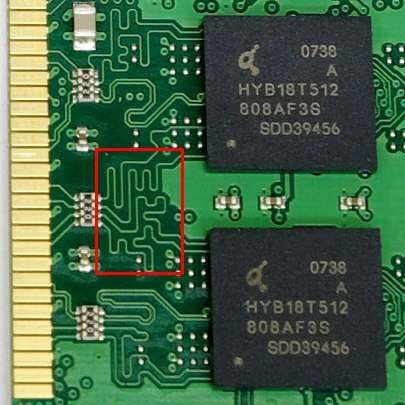
\includegraphics[height=0.5\textheight]{img/\jobname/length_equiv.jpg}
        \end{figure}
    \end{enumerate}
\end{frame}


\begin{frame}{... и длины дорожек должны быть равны!}
    \begin{enumerate}
        \item Что нам мешает?
        \begin{enumerate}
            \item Противостояние тактовая частота --- скорость света
            \item «Широкая» шина
        \end{enumerate}
        \pause
        \item \alert{Решение: снизить разрядность шины, а если нужно передавать больше данных --- сделать несколько независимых (асинхронных) параллельных шин.}

        На <<узкой>> шине выровнять дорожки легче. До сих пор <<держатся>> параллельными дорожки к ОЗУ, и то с оговорками (RAS/CAS), но об этом позже
    \end{enumerate}
\end{frame}

\section{Внутренняя шина PCI Express}

\begin{frame}{PCI Express: Root Complex}
	\begin{figure}
        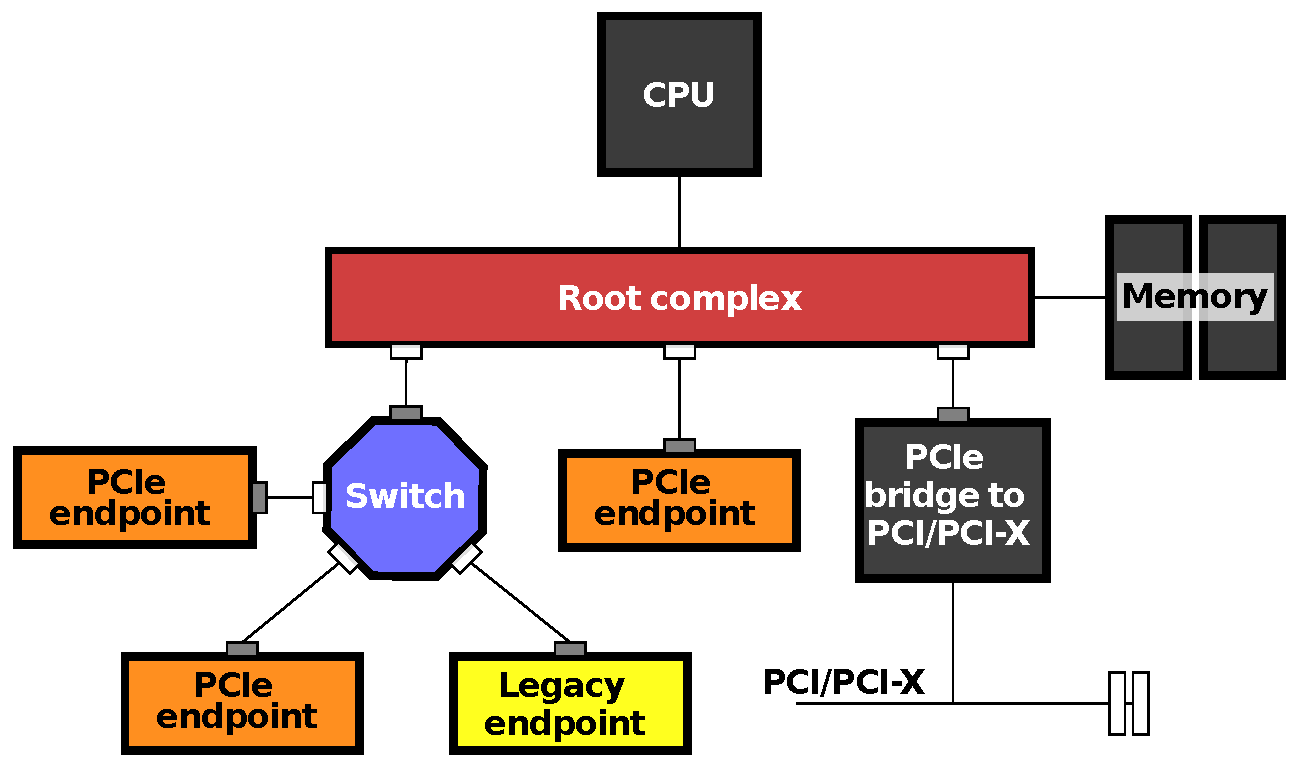
\includegraphics[height=0.5\textheight]{img/\jobname/Example_PCI_Express_Topology.pdf}
    \end{figure}
    \begin{itemize}
        \item Северный мост трансформироавлся в \href{https://en.wikipedia.org/wiki/Root_complex}{Root Complex}, в современные процессоры обычно встраивается на кристалл, реже --- отдельным кристаллом в том же корпусе
        \item Южный мост «размазался»
        \item Некоторые традиционно «не периферийные» устройства, например ПЗУ (точнее ППЗУ) доступны через последовательную шину
    \end{itemize}
\end{frame}

\begin{frame}{PCI Express: Полосы, Совместимость разъёмов разной ширины}
	\begin{figure}
        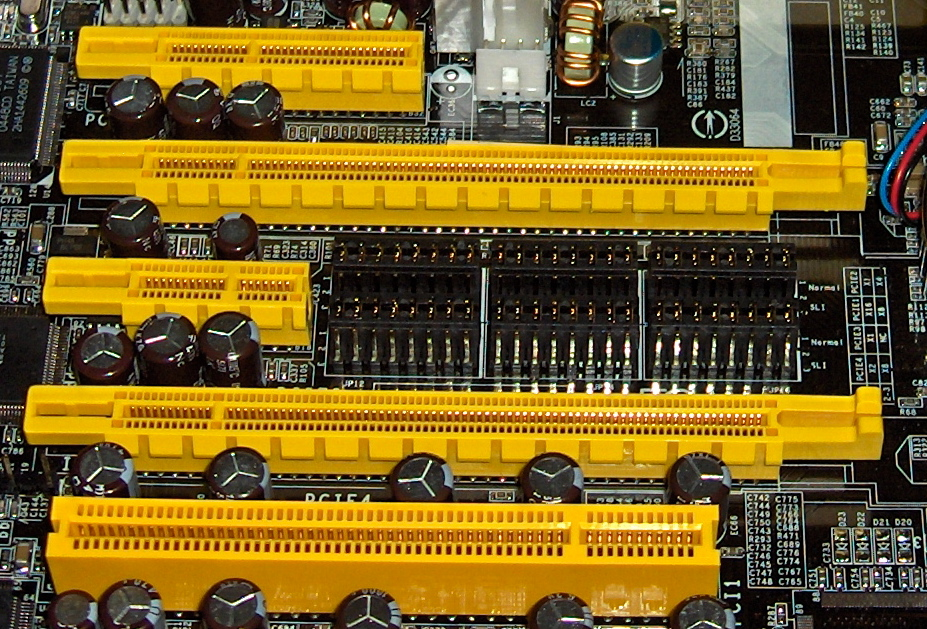
\includegraphics[height=0.5\textheight]{img/\jobname/PCI-E_PCI_slots.jpg}
        \caption{\href{https://en.wikipedia.org/wiki/PCI_Express}{Разные разъёмы PCI-E (+ 1 PCI)}}
    \end{figure}
    \begin{itemize}
        \item Разные версии стандарта --- разные скорости
        \item Передача данных \emph{пакетами}, в зависимости от длины разъёма --- от 1 до 16 пакетов одновременно
        \begin{itemize}
            \item Устройства и разъёмы разной длины [обычно] совместимы друг с другом, если их можно соединить механически
            \begin{itemize}
                \item Короткое устройство будет работать в длинном разъёме
                \item Длинное устройство может иметь вырезы на контактной площадке, либо вставляться в «открытый» разъём
            \end{itemize}
        \end{itemize}
    \end{itemize}
\end{frame}

\begin{frame}{PCI Express: Скорости}
    \begin{figure}
        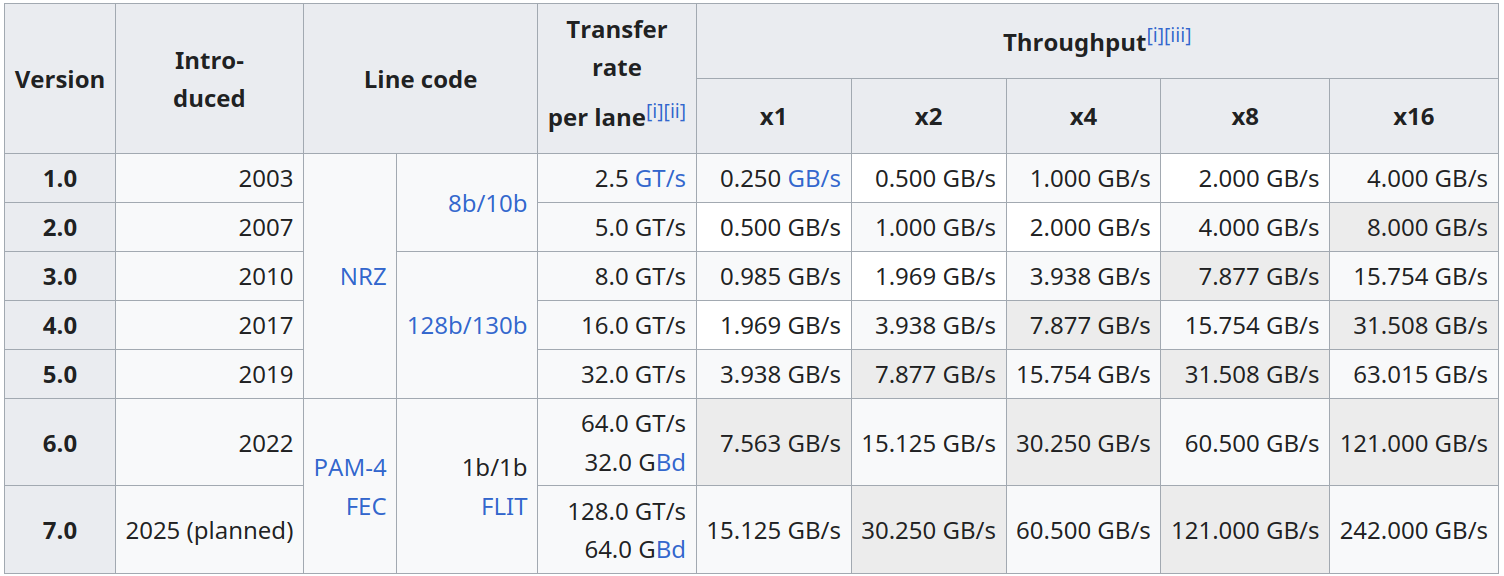
\includegraphics[height=0.5\textheight]{img/\jobname/PCI-E_Speeds.png}
        \caption{Скорости PCI Express по данным \href{https://en.wikipedia.org/wiki/PCI\_Express\#History\_and\_revisions}{Википедии} и \href{https://web.archive.org/web/20131019114456/http://www.pcisig.com/news_room/faqs/pcie3.0\_faq/PCI-SIG\_PCIe\_3\_0\_FAQ\_Final\_07102012.pdf}{Peripheral Component Interconnect Special Interest Group}}
    \end{figure}
\end{frame}

\begin{frame}{Mini PCI Express, mSATA и M.2}
    \begin{figure}
        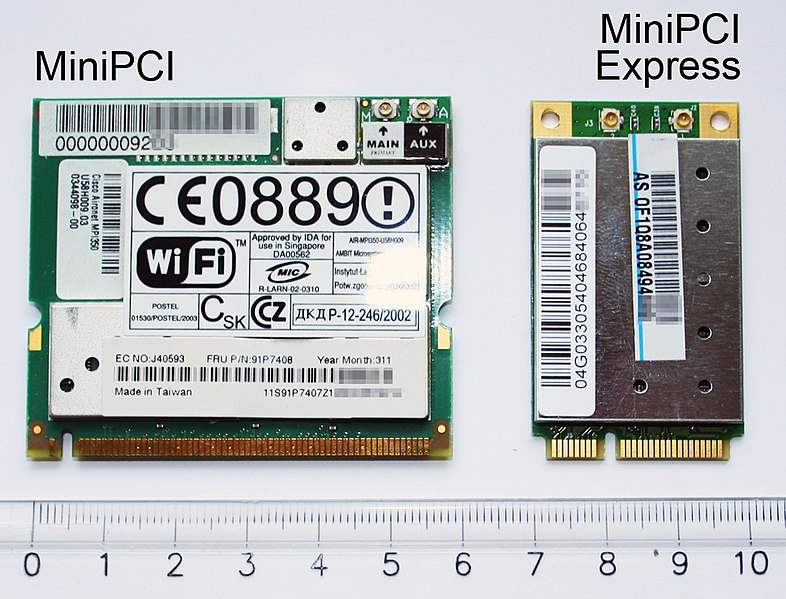
\includegraphics[height=0.35\textheight]{img/\jobname/MiniPCI_and_MiniPCI_Express_cards.jpg}
        \caption{\href{https://en.wikipedia.org/wiki/PCI_Express\#MINI-CARD}{Mini PCI \& Mini PCI-E}}
    \end{figure}
    \begin{figure}
        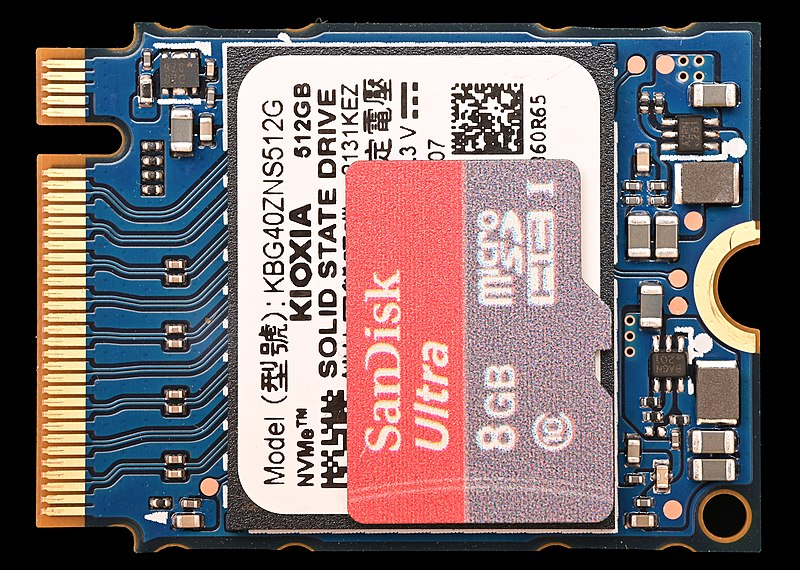
\includegraphics[height=0.25\textheight]{img/\jobname/M.2_Carg.jpg}
        \caption{\href{https://en.wikipedia.org/wiki/M.2\#Form_factors_and_keying}{M.2}
        \href{https://en.wikipedia.org/wiki/M.2\#/media/File:SATA_Express_interface.svg}{использует одинаковый электический и сигнальный интерфейсы с mSATA},\\это типичная практика, и об этом ниже
        }
    \end{figure}
\end{frame}

\section{Интерфейсные шины USB и Thunderbolt}

\subsection{Universal Serial Bus}

\begin{frame}{Universal Serial Bus}

\begin{itemize}
    \item Используется с середины 1990-х
    \item Идеи:
    \begin{itemize}
        \item Универсальность
        \item Возможность под/отключения на ходу
        \item Механически прочный разъём c мощным питанием
        \item \alert<2->{Последовательная передача данных (1 линия на 2 контактах и 2 проводах)}
        \item Изначально — не очень высокая скорость: у хорошо настроенного параллельного порта IEEE 1284 (LPT) скорость выше, чем у USB 1.X
    \end{itemize}
    \pause

    \item За более, чем 25-летнюю историю:
    \begin{itemize}
        \item \href{https://en.wikipedia.org/wiki/USB\#Connector_type_quick_reference}{Не смог сохранить простоту}
        \item \alert{USB 3+ по сравнению с USB 2- дополнился двумя высокоскоростными линиями данных}, \href{https://electronics.stackexchange.com/a/587798}{т.е. стал уже не совсем последовательным}
        \item Потеснил или вытеснил почти все «повседневные» цифровые интерфейсы: COM (RS-232), LPT, AT и PS/2, Twain, FireWire\ldots
    \end{itemize}
\end{itemize}

\end{frame}

\begin{frame}{USB DisplayPotr Alt Mode}
    USB 3.1+ c разъёмом Type C позволяют инкапсулировать протокол DisplayPort
\end{frame}

\subsection{Thunderbolt}

\begin{frame}{Thunderbolt 1, 2}
    \begin{columns}
        \begin{column}{0.5\textwidth}
            \begin{itemize}
                \item Высокоскоростной интерфейс, появился в 2011
                \item Использовал разъём Mini DisplayPort и был совместим с протоколом DisplayPort на уровне электрических контактов и сигналов
                \item Мог инкапсулировать DisplayPort или работать в режиме DisplayPort
                \item \alert{Мог даже инкапсулировать PCI Express} (через него даже подключали внешние графические адаптеры)
                \item Версии 1 и 2 отличались скоростями и версиями инкапуслируемых протоколов
            \end{itemize}
        \end{column}
        \begin{column}{0.5\textwidth}
            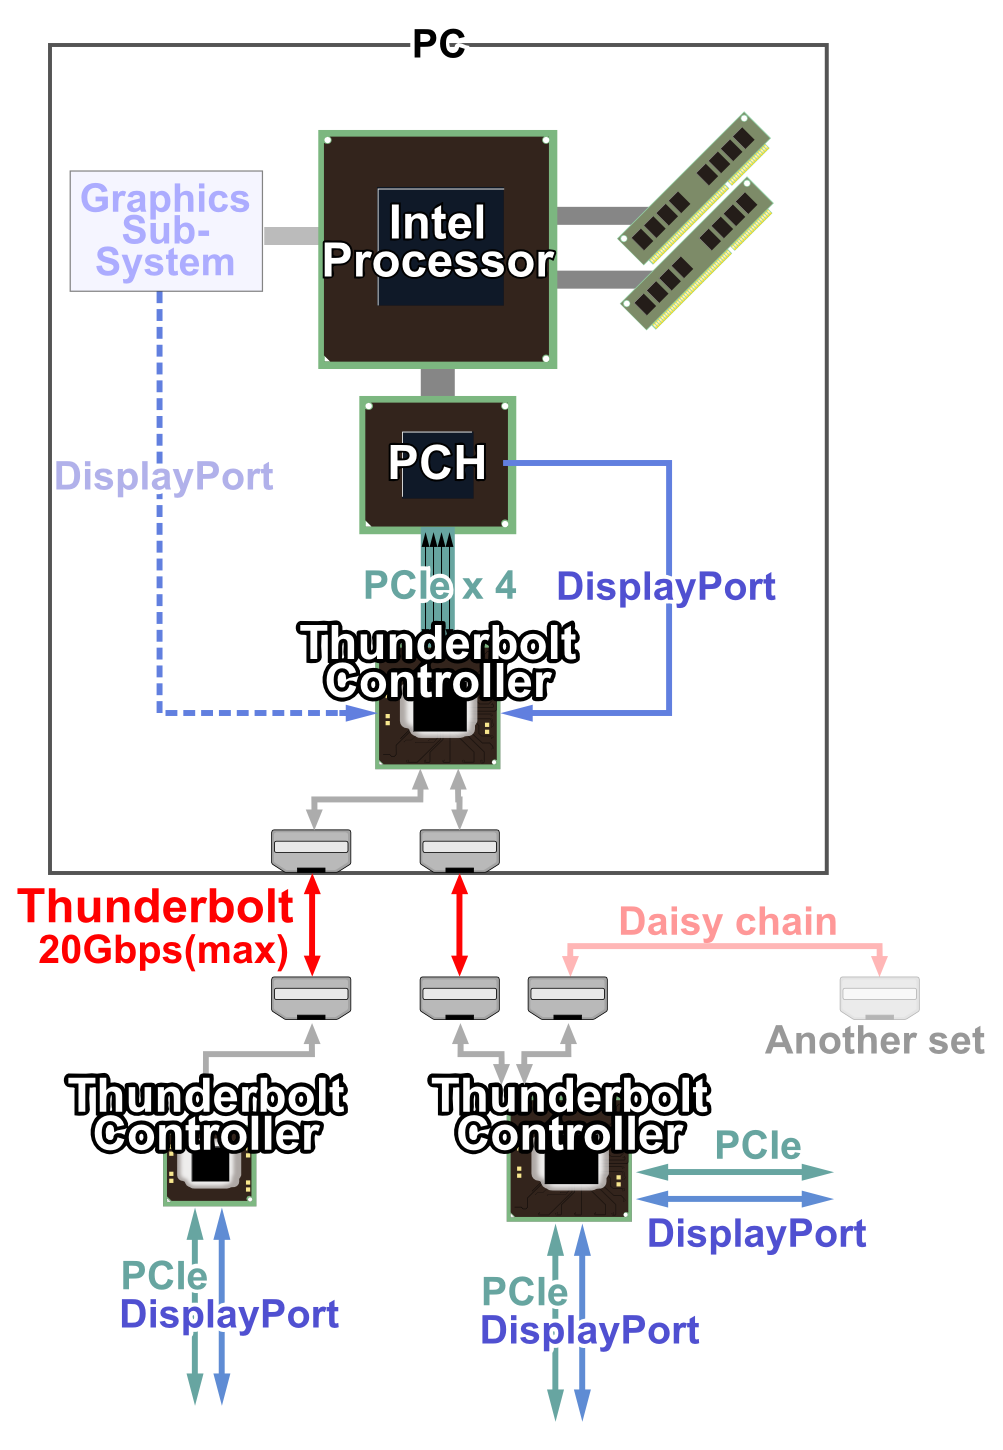
\includegraphics[height=0.8\textheight]{img/\jobname/Thunderbolt_1.png}
        \end{column}
    \end{columns}
\end{frame}

\begin{frame}{Thunderbolt 3}
    \begin{itemize}
        \item Использует разъём Type C
        \item Практически является расширением USB 3
        \item \href{https://market.yandex.ru/product--usb-kontsentrator-baseus-thunderbolt-c-pro-cahub-l0g-razemov-5/424956176}{Поддерживает параллельную работу двух портов} (почти как PCI Express lanes), как одного ускоренного (расстояние стандартизовано)
    \end{itemize}
\end{frame}

\subsection{Современные USB и Thunderbolt}

\begin{frame}{Кто на ком основан?..}
    USB 3.2 $\rightarrow$ Thunderbolt 3 $\rightarrow$ USB 4 (ещё быстрее + открытая спецификация инкапсуляции PCI Ecpress)  \ldots Thunderbolt 4, 5

    Общая тенденция к тому, что оба протокола унифицируются друг с другом, ускоряются и добавляют больше функциональности
\end{frame}

\section*{}

\begin{frame}{Упражнения и вопросы}
	\begin{block}{Упражнения}
		\begin{itemize}
			\tightlist
			\item
			Попытайтесь идентифицировать все компьютерные разъёмы, которые вы можете встретить
		\end{itemize}
	\end{block}

	\begin{block}{Вопросы}
		\begin{itemize}
			\tightlist
            \item
            Что такое Root Complex?
            \item
            В чём смысл использования последовательных шин расширения?
            \item
            Приведите примеры различных протоколов, использующих одинаковые электрические и сигнальные интерфейсы
		\end{itemize}
	\end{block}
\end{frame}

\postamble
\end{document}
